\documentclass[a4paper,12pt]{article}
\usepackage[utf8]{inputenc}
\usepackage{graphicx}
\usepackage{float}

%opening
\title{TOK: Are some things unknowable?}
\author{Terry Qi}

\begin{document}

\maketitle
\begin{enumerate}
 \item G\"odel's Incompleteness Theorem
 \item Double Pendulum
 \item Progress bars - The halting problem
\end{enumerate}

\begin{figure}[h!]
 \centering
 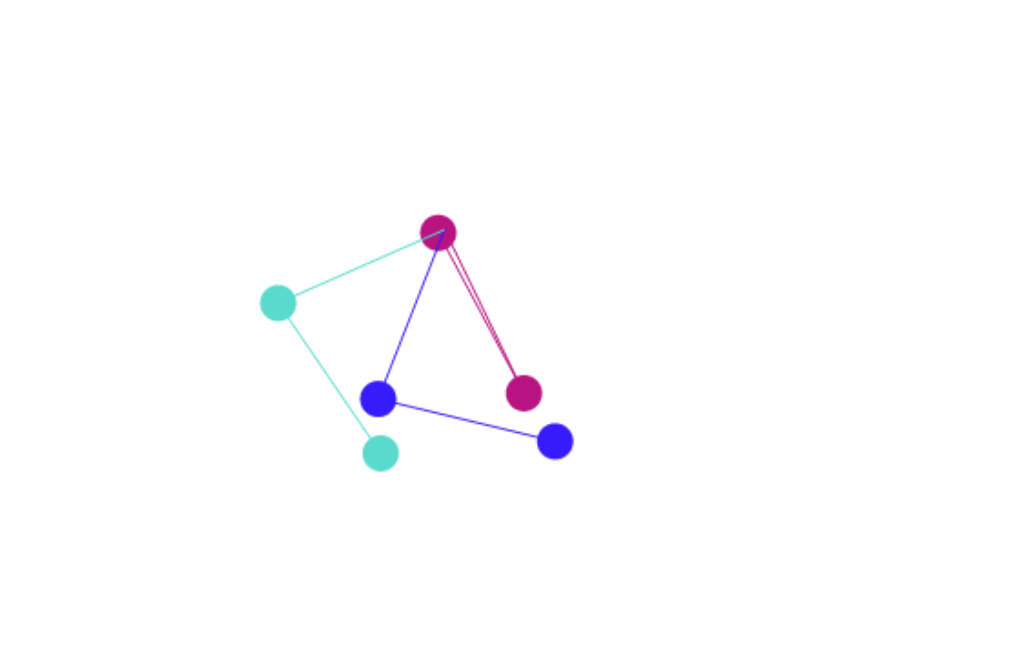
\includegraphics[scale=0.25]{dpend.png}
 \caption{Three Double Pendulum}
\end{figure}

\begin{figure}[h!]
 \centering
 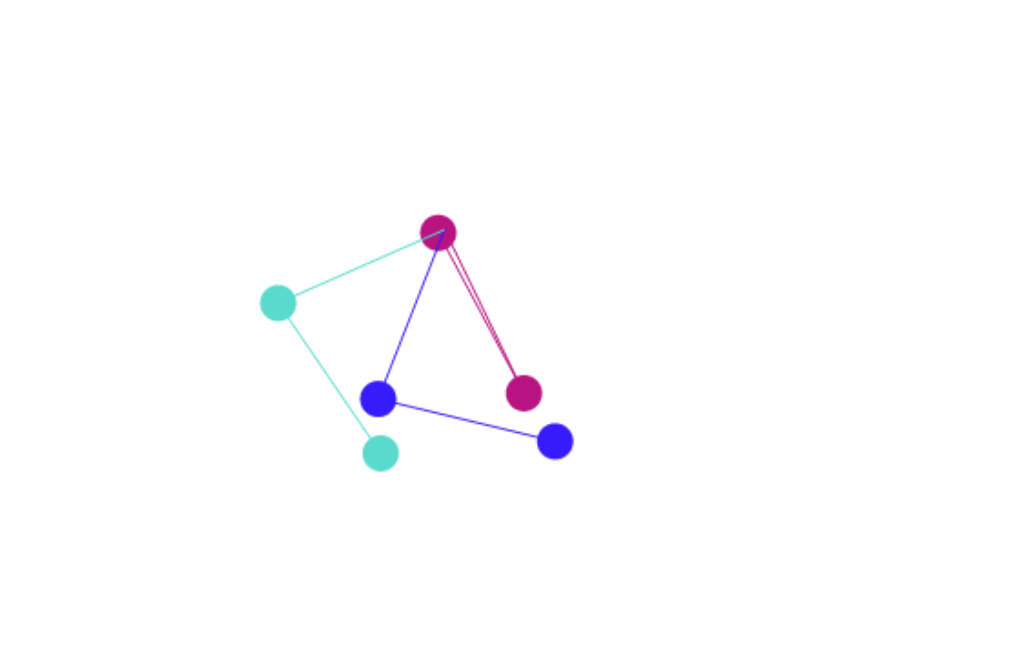
\includegraphics[scale=0.25]{dpend.png}
 \caption{Three Double Pendulums}
\end{figure}

\begin{figure}[h!]
 \centering
 
\includegraphics[scale=0.35]{progress.png}
 \caption{A progress bar}
\end{figure}



\newpage

\paragraph{1}
\paragraph{2}
\paragraph{3}

\end{document}
